\documentclass{article}

\usepackage[left=1in, right=1in, top=1in, bottom=1in]{geometry}

\usepackage{setspace}
\usepackage{fancyhdr}
\usepackage{hyperref}
\usepackage{amsthm}
\usepackage{amssymb}
\usepackage{multirow}
\usepackage{enumitem}
\usepackage{graphicx}
\usepackage{makecell}
\usepackage{booktabs}
\usepackage{titlesec}
\usepackage{amsmath}
\usepackage{pdfpages}
\usepackage{enumitem}
\usepackage{caption}

\setcounter{secnumdepth}{4}

\hypersetup{
    colorlinks=true,     
    urlcolor=magenta
}

\renewcommand{\qedsymbol}{\rule{0.7em}{0.7em}}

\newlength\tindent
\setlength{\tindent}{\parindent}
\setlength{\parindent}{0pt}
\renewcommand{\indent}{\hspace*{\tindent}}
\setlength{\parskip}{0em}

\newenvironment{blockquote}{%
  \par%
  \vskip1em
  \leftskip=2em\rightskip=2em%
  \noindent\ignorespaces}{%
  \par\vskip1em}

\newenvironment{blockquote2}{%
	\par%
	\vskip1em
	\leftskip=4em\rightskip=4em%
	\noindent\ignorespaces}{%
	\par\vskip1em}

\pagestyle{fancy}
\fancyhf{}
\fancyhead[LO]{STA5176}
\fancyhead[RO]{Kyle Ligon}
\fancyfoot[LO]{Chapter 8 and 9}
\fancyfoot[RO]{\thepage}
 
\renewcommand{\headrulewidth}{0.5pt}
\renewcommand{\footrulewidth}{0.5pt}

\begin{document}
\section*{Chapter 8 and 9 Homework}
\subsection*{Due 3-18-2018}
\subsubsection*{Problem 9.13}
\subsubsection*{ a) Assess ANOVA assumptions using the graph from PROC MIXED.}

In order to proceed with ANOVA, we must check for the following pieces:
\begin{itemize}[leftmargin=+.5in]
 	\item[$\bullet$] No obvious pattern in our Residual Scatterplot
	\item[$\bullet$] Normal shape to the Residual Histogram.
 	\item[$\bullet$] Residuals fit along the linear prediction of our Actual "Normality" to the Theoretical Normal Model.  
\end{itemize}

Since there is no readily observable pattern in our residuals, our distribution is mound shaped, and our Residuals fit the along the Q-Q plot(although, there may be evidence of a right skew), we will proceed with ANOVA to see if at least one mean is different.  

\begin{figure}[h]
\centering
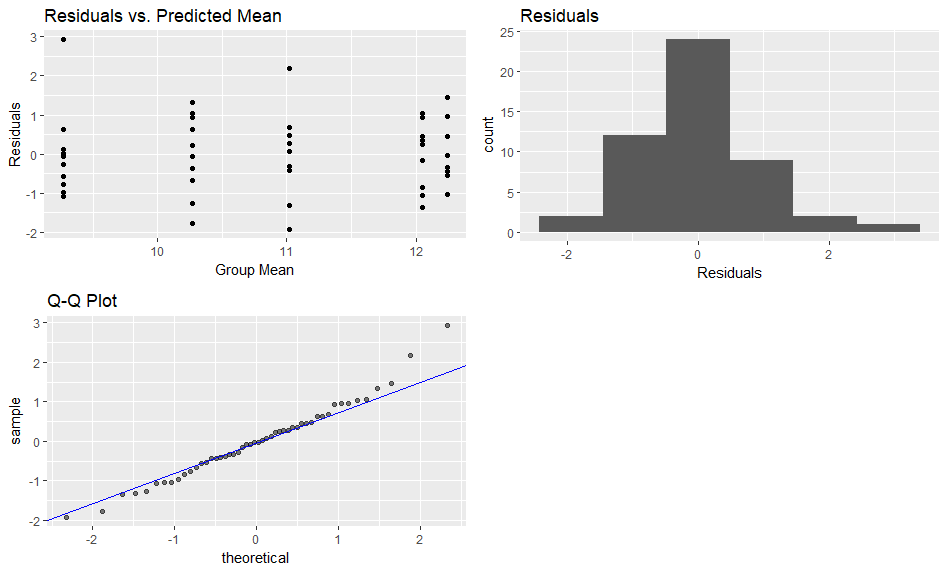
\includegraphics[width = 1.0\textwidth]{AnovaCheck.png}
\end{figure}

\pagebreak

\subsubsection*{ b) Perform ANOVA to determine if there is a difference among the five weight-reducing agents, $\alpha$ = 0.05.} 
\begin{table}[ht]
\caption{ANOVA Table for Weight Loss Study}
\centering
\begin{tabular}{l c c c c c}
\hline\hline
Row Names & SS & df & MS & F & P-Value \\ [0.5ex] 
\hline
Treatments (T) & 61.618 & 4 & 15.4045 & 15.6805 & 4.16x$10^{-8}$ \\
Error (E) & 44.207 & 45 & 0.9824 & \\
Total & 105.825 & 49 &  \\ [1ex]
\hline
\end{tabular}
\label{table:nonlin}
\end{table}

Hypotheses:
\begin{blockquote}
$H_{0}$: $\mu_{a1}$ = $\mu_{a2}$ = $\mu_{a3}$ = $\mu_{a4}$ = $\mu_{s}$ \\
$H_{1}$: At least one mean is different.  
\end{blockquote}
Test Statistic:
\begin{blockquote}
F = 15.6805
\end{blockquote}
Rejection Region:
\begin{blockquote}
Reject $H_{0}$ if $F_{0} > F_{\alpha, 4, 45}$ \\
$F_{0.95, 4 , 45} = 5.72$
\end{blockquote}
Conclusion/Interpretation:
\begin{blockquote}
Since our $F_{0} > 5.72$, there is strong enough evidence to support rejecting the null hypothesis that the means are the same.  The data provided does suggest at least one mean is different from the rest.  
\end{blockquote}


\subsubsection*{ c) Determine significantly different pairs using Tukey's W with $\alpha$ = 0.05}
\begin{blockquote}
To find which groups are different from each other, we will utilize Tukey's W to check which means are different from one another.  We will verify this by checking which one's p-values are less than 0.05 after using the TukeyHSD test on our ANOVA Model in R.  
\end{blockquote}
Conclusion/Interpretation
\begin{blockquote}
With our Tukey W test being run, the differences lie in the following means:
\end{blockquote}

\begin{itemize}[leftmargin=+0.5in]
	\item[$\bullet$] S differs with $A_{1}$, $A_{2}$, and $A_{4}$
	\item[$\bullet$] $A_{3}$ differs with $A_{1}$ and $A_{4}$
\end{itemize}

\pagebreak

\subsubsection*{ d) Determine which, if any, of the new agents have significantly larger mean weight loss as compared to the standard agent; $\alpha$ = 0.05}

\begin{blockquote} 
Using s as our control, we will performs Dunnett's test to determine if there's a significantly larger difference with the new agents.  The first step in checking out if any of the new agents are yielding better weight loss results is to find Dunnett's D.  
\end{blockquote}

\begin{eqnarray}
D = d_{\alpha}(k,v)\sqrt{\frac{2s^{2}_{W}}{n}} \nonumber \\ 
D = d_{0.05}(4,45)\sqrt{\frac{2(0.982)}{10}} \nonumber \\
D = 2.23\sqrt{\frac{1.964}{10}} \nonumber \\
D = 2.23(0.4432) \nonumber \\
D = 0.9888 \nonumber
\end{eqnarray}

\begin{table}[h]
\caption{Dunnett's Control Test}
\centering
\begin{tabular}{c c c c}
\hline\hline
Treatment & $\bar{y}_{i}-\bar{y}_{c}$ & Comparison & Conclusion \\ [0.5ex] 
\hline
a1 & 2.78 & $>$ D & Greater Than Control \\
a2 & 1.75 & $>$ D & Greater Than Control \\
a3 & 1.00 & $>$ D & Greater Than Control \\ 
a4 & 2.97 & $>$ D & Greater Than Control \\ [1ex]
\hline
\end{tabular}
\label{table:nonlin}
\end{table}    

Conclusion/Interpretation:
\begin{blockquote}
All four of the agents are statistically significant. Thus, we can reject the null hypotheses that the difference in weight loss metrics between the original agent(s) and the new agents($a_{1}, a_{2}, a_{3},$ and $a_{4}$) is zero.  Each of the new agents appear to have an increase in weight loss over the agent s.    
\end{blockquote}

\subsubsection*{9.17 - construct the contrasts for the following:}
\subsubsection*{a) Compute the mean for the standard agent to the average of the means for the four new agents}
\begin{equation}
\hat{l} = \bar{y_{S}} - \frac{1}{4}\bar{y}_{A_{1}} -\frac{1}{4}\bar{y}_{A_{2}} -\frac{1}{4}\bar{y}_{A_{3}} -\frac{1}{4}\bar{y}_{A_{4}} \nonumber
\end{equation}

\subsubsection*{b) Compare the mean for the agents with counseling to those without counseling. (Ignore the standard)}
\begin{equation}
\hat{l} = \bar{y}_{A_{1}} + \bar{y}_{A_{3}} - \bar{y}_{A_{2}} -\bar{y}_{A_{4}} \nonumber
\end{equation}
\subsubsection*{c) Compare the mean for the agents with exercise to those without exercise.}
\begin{equation}
\hat{l} = \bar{y}_{A_{1}} + \bar{y}_{A_{2}} - \bar{y}_{A_{3}} - \bar{y}_{A_{4}} \nonumber 
\end{equation}
\subsubsection*{d) Compare the mean for the agents with counseling to the standard.}
\begin{equation}
\hat{l} = \bar{y}_{A_{1}} + \bar{y}_{A_{3}} - 2\bar{y_{S}} \nonumber
\end{equation}


\subsubsection*{8.27 a) Assess ANOVA assumptions using the graph from PROC MIXED}
In order to proceed with ANOVA, we must check for the following pieces:
\begin{itemize}[leftmargin=+.5in]
 	\item[$\bullet$] No obvious pattern in our Residual Scatterplot
	\item[$\bullet$] Normal shape to the Residual Histogram.
 	\item[$\bullet$] Residuals fit along the linear prediction of our Actual "Normality" to the Theoretical Normal Model.  
\end{itemize}

There appears to be a pattern in the residuals.  The best way to describe the pattern is a increasing fan shape at the edges.  There is an increase in the residuals as you are on the extremes of the means of each group.  Finally, a pattern in the Q-Q plot has this sample data straying from the Normal model by mismatching the Normal model outside of the -1 and + 1.5 standard deviations.     


\begin{figure}[h]
\centering
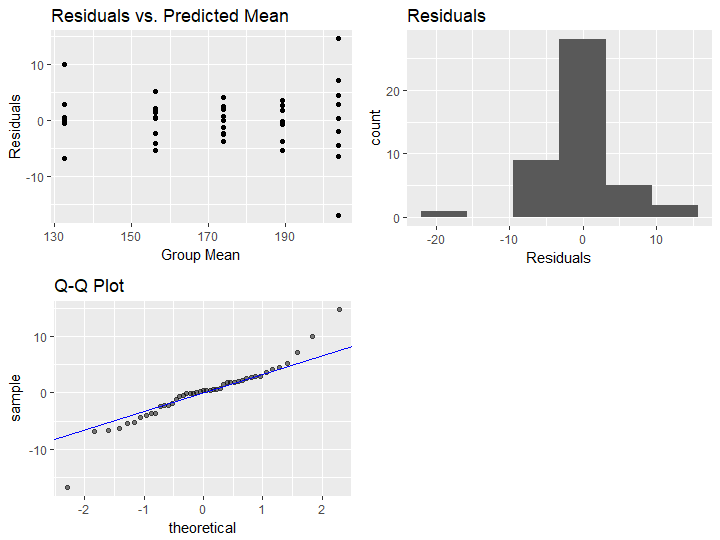
\includegraphics[width = 0.8\textwidth]{827AnovaCheck.png}
\end{figure}


\subsubsection*{b) Run an ANOVA on the data to see if there is a difference in the suppliers}
\begin{table}[ht]
\caption{ANOVA Table for Supplier's Variability in Power}
\centering
\begin{tabular}{l c c c c c}
\hline\hline
Row Names & SS & df & MS & F & P-Value \\ [0.5ex] 
\hline
Suppliers (S) & 28024 & 4 & 7006 & 865.9 & $<$ 2x$10^{-16}$ \\
Error (E) & 1054 & 40 & 26 & \\
Total & 29078 & 44 &  \\ [1ex]
\hline
\end{tabular}
\label{table:nonlin}
\end{table}
Hypotheses:
\begin{blockquote}
$H_{0}: \mu_{S1} = \mu_{S2} = \mu_{S3} = \mu_{S4} = \mu_{S5}$ \\
$H_{1}:$ At least one mean is different.  
\end{blockquote}
\pagebreak
Test Statistic:
\begin{blockquote}
F = 865.9
\end{blockquote}

Rejection Region:
\begin{blockquote}
Reject $H_{0}$ if $F_{0} > F_{\alpha,4,20}$
$F_{0.05,4,25}$ = 5.80
\end{blockquote}

Conclusion/Interpretation:
\begin{blockquote}
With a test statistic greater than the rejection bound, there does seem to extreme enough evidence to reject the null hypothesis that the means are equal.  It does appear that at least one mean is different.  
\end{blockquote}

\subsubsection*{c) Perform a Kruskal-Wallis test to determine if there is a difference among the suppliers; $\alpha$ = 0.05}
Hypothesis:
\begin{blockquote}
$H_{0}$: There is no difference among the five suppliers with respect to median Variability in Power. \\
$H_{1}$: At least one of the five suppliers' medians differs from the others.   
\end{blockquote}

Test Statistic:
\begin{blockquote}
H = 41.596 with 4 degrees of freedom and a p-value of 2.023x$10^{-8}$
\end{blockquote}

Rejection Region:
\begin{blockquote}
We will reject if H $> \chi_{0.05, 4}^{2}$ \\
$\chi_{0.05, 4}^{2} = 9.488$
\end{blockquote}

Conclusion/Interpretation
\begin{blockquote}
Since our Test Statistic is greater than 9.488, we have significant evidence to reject the Null Hypothesis that the all the medians are the same.  There does appear to be at least one median that is different than the rest.   
\end{blockquote}

\subsubsection*{d) Compare the results from b) and c) - which analysis would you say is correct?}
Reasoning:
\begin{blockquote}
In determining which analysis to agree with, I am hesitant to base decisions on the ANOVA approach due to its pattern in its residuals.  Additionally, such a small sample set of 9 observations per Supplier has me raising an eye brow at the thought of trusting an ANOVA test's results.  Finally, the Q-Q plot's lack of fidelity to the theoretical Normal distribution, particularly at the extreme ends of the linear model, has me doubting even more. Thus, the non-parametric approach with Kruskal-Wallis is what I would base my decision making on.  
\end{blockquote}

\subsubsection*{e) Determine significantly different pairs using Tukey's W with $\alpha$ = 0.05.}
To find which groups are different from each other, we will utilize Tukey's W to check which means are different from one another.  We will verify this by checking which one's p-values are less than 0.05 after using the TukeyHSD test on our ANOVA Model in R.  \\ 
\pagebreak
Conclusion/Interpretation:
\begin{blockquote}
With our Tukey W test being run, the differences lie in the following means:
\begin{itemize}[leftmargin=+0.5in]
	\item[$\bullet$] All the Suppliers are different with each other.  They all have a p-value less than 0.05.  
\end{itemize}

\end{blockquote}
\begin{table}[h]
\caption{Tukey HSD Test for Variability in Power per Supplier}
\centering
\begin{tabular}{c c c c c}
\hline\hline
Supplier & diff & lower bound & upper bound & p-value \\ [0.5ex] 
\hline
S3-S4 & 23.6667 & 16.7516 & 30.5772 & $3.6567x10^{-11}$ \\
S2-S4 & 41.3889 & 34.4783 & 48.2994 & $4.6363x10^{-13}$ \\
S1-S4 & 56.5333 & 49.6228 & 63.4439 & $4.6363x10^{-13}$ \\ 
S5-S4 & 71.3333 & 64.4228 & 78.2439 & $4.6363x10^{-13}$ \\ 
S2-S3 & 17.7222 & 10.8117 & 24.6328 & $6.5207x10^{-13}$ \\
S1-S3 & 32.8667 & 25.9561 & 39.7772 & $4.6829x10^{-13}$ \\
S5-S3 & 47.6667 & 40.7561 & 54.5772 & $ 4.6363x10^{-13}$ \\
S1-S2 & 15.1444 & 8.2339 & 22.0550 & $1.9784x10^{-06} $ \\
S5-S2 & 29.9444 & 23.0339 & 36.8550 & $5.0204x10^{-13} $ \\
S5-S1 & 14.8000 & 7.895 & 21.7106 & $3.1290x10^{-06}$ \\ [1ex]
\hline
\end{tabular}
\label{table:nonlin}
\end{table}    


\subsubsection*{f) Determine significantly different pairs using the Kruskal-Wallis approach using $\alpha$ = 0.05.  }

\begin{table}[h]
\caption{Table of Suppliers' Mean Ranks}
\centering
\begin{tabular}{c c c c c}
\hline\hline
Supplier 1 & Supplier 2 & Supplier 3 & Supplier 4 & Supplier 5 \\ [0.5ex] 
\hline
33.00 & 23.00 & 14.00 & 5.00 & 40.22 \\ [1ex]
\hline
\end{tabular}
\label{table:nonlin}
\end{table}    

Rejection Region:
\begin{blockquote}
With the means of the ranks calculated for each group, we will calculate the Rejection bound for the KW test.  
\end{blockquote}

\begin{eqnarray}
KW \approx \frac{q_{\alpha}(t,\infty)}{\sqrt{2}}\sqrt{\frac{n_{T}(n_{T}+1)}{12}\Big(\frac{1}{n_{i}}+\frac{1}{n_{j}}\Big)} \\ \nonumber
KW \approx \frac{3.86}{\sqrt{2}}\sqrt{\frac{45(46)}{12}\Big(\frac{1}{9}+\frac{1}{9}\Big)} \\ \nonumber 
KW \approx 2.7294(6.1914) \\ \nonumber
KW \approx 16.8988 \\ \nonumber
\end{eqnarray}

\pagebreak
\begin{table}[h]
\caption{Tukey HSD Test for Variability in Power per Supplier}
\centering
\begin{tabular}{c c c}
\hline\hline
Supplier Difference & $|R_{i}-R_{j}|$ & Conclusion \\ [0.5ex] 
\hline
Supplier1-Supplier2 & $|33.00-23.00| = 10$ & Not Significantly Different \\
Supplier1-Supplier3 & $|33.00-14.00| = 19$ & Significantly Different \\
Supplier1-Supplier4 & $|33.00-5.00| = 28.00$ & Significantly Different\\ 
Supplier1-Supplier5 & $|33.00-40.22| = 7.22$ & Not Significantly Different\\ 
Supplier2-Supplier3 & $|23.00-14.00| = 9$ & Not Significantly Different \\
Supplier2-Supplier4 & $|23.00-5.00| = 18.00$ & Significantly Different \\
Supplier2-Supplier5 & $|23.00-40.22|= 17.22$ & Significantly Different \\
Supplier3-Supplier4 & $|14.00-5.00| = 9.00$ & Not Significantly Different\\
Supplier3-Supplier5 & $|14.00-40.22| = 26.22$ & Significantly Different\\
Supplier4-Supplier5 & $|5.00-40.22| = 35.22$ & Significantly Different \\ [1ex]
\hline
\end{tabular}
\label{table:nonlin}
\end{table}    




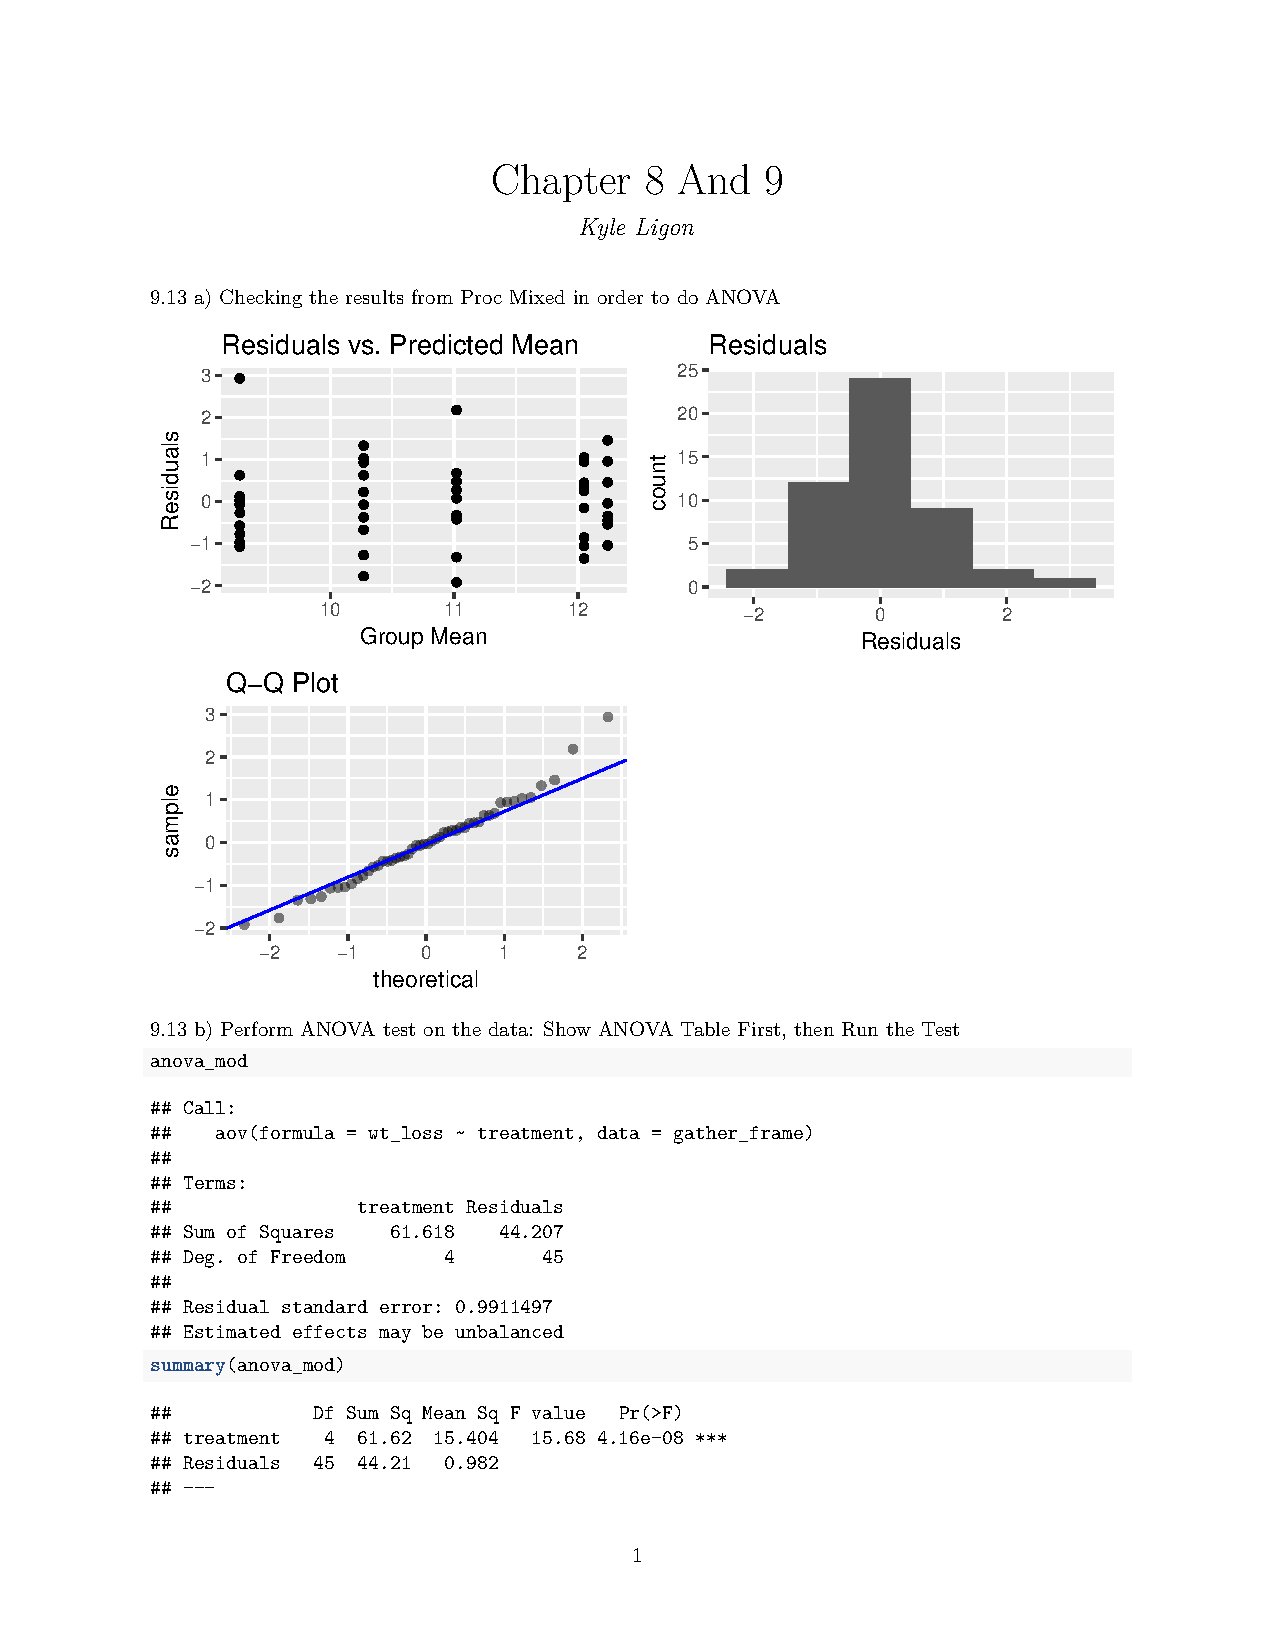
\includepdf[pages=-]{Chapter_8_And_9.pdf}
\end{document}



